%------------------------------%
% \chapter{Privacy and Ethics in Web of Socially Intelligent Agents}
\chapter{Reasoning about Values and Ethics}
\label{chap:ainur}
%------------------------------%

This chapter describes \frameworkAinur, our approach to 
design ethical SIPAs that understand value preferences and
reason about them, and its empirical evaluation.

\section{Introduction}

A \emph{social machine} is characterized as a sociotechnical system comprising of social entities such as humans and technical components such as software jointly involved in the physical realization of a process \citep{Smart+14:social-machines,WWW-16:IOSE}. 
In the original conception of social machines, humans engage in the creative elements of this realization process, whereas technical components  administer the process \citep{Berners-Lee-99:Weaving}.

The conception of social machines has been gaining significant attention from academia and industry in recent years. 
Prominent social web applications such as Wikipedia, Facebook, Twitter, Instagram, and Snapchat are examples of social machines.
The very nature of social machines dictates that privacy be a key concern in their design. 
Whereas current methods for designing privacy into (social) web applications emphasize technology-centric notions such as authentication \citep{Ruoti-WWW2015-AuthenticationMelee} and access control \citep{Paci-CSUR2018-CollaborativeAccessControl}, they struggle to incorporate social mechanisms to control the threats to privacy \citep{Hendler-AI2010-SocialMachine}. 
Such social mechanisms are of paramount importance in realizing privacy respecting social machines.

% \citet{schwartz2012overview} defines values as guiding principles of humans \mps{reads odd}. 
Values are broad motivational goals or ideals worth pursuing for humans \citep{schwartz2012overview,Dechesne-AIL13-Norms+Values}.
Ethicists subsume ethics in the theory of values \citep{Friedman-2008-value-sensitive-design}. 
Privacy is regarded as a value with an ethical import \citep{Langheinrich-01:privacy,Taylor-2002-PrivacyAutonomy}. 
% 
As envisioned, social machines facilitate natural interactions among autonomous parties (humans and organizations) as opposed to the predominant style of supporting social interactions via centralized servers (ranging from email servers to social network sites).
% Privacy considerations will be\mps{redo the sentence} far more nuanced\mps{why?} than what they are today if we are to realize the web as a social machine.

On the backdrop of privacy concerns and a rising number of privacy breach incidents, new regulations and standards such as the General Data Protection Regulation (GDPR) \citep{gdpr-18} are being introduced. 
\citet{spiekermann2009enggprivacy} suggest that to ensure effective implementation of privacy standards, it is necessary for engineers to design privacy-preserving systems that allow their users to control access to their private information. 
However, giving control to users raises two key concerns. 
First, does the information the users share on the web accord with their values? 
Second, does this sharing of information promote or demote any values for any other users concerned with the information? 
% 
More often than not these concerns are not addressed when users today make sharing decisions, as there is an excessive burden of decision making on them. 
A \fsl{SIPA} can help a user in decision making and sometimes automate it. 

We seek to design a social machine in which each user is supported by an (artificial) personal agent \citep{Murukannaiah-AAMAS14-Xipho}. 
These agents interact with each other to facilitate creativity in social machines. 
We refer to such an agent as a socially intelligent personal agent (SIPA). 
Importantly, SIPAs in our setting understand values and act ethically. 
We emphasize privacy as a value in our examples and experiments, as privacy has an ethical import \citep{Friedman-2008-value-sensitive-design}. 
Whereas much of the existing literature on artificial intelligence focuses on rational decision-making by agents, we consider the problem of designing agents that act according to users' values and preferences among those values.

%\subsection{Values}
%
%The concept of \fsl{value} has two main connotations: one is about economic worth of something and the other, more broadly, refers to what people consider important in their lives \citep{Friedman-2008-value-sensitive-design}. 
%We adopt the later connotation in this work.
%
%Values are mostly universal across human societies as stated by \citet{schwartz2012overview} and \citet{rokeach1973nature}. 
%The values in Schwartz's \citep{schwartz2012overview} work are broad motivational goals, such as stimulation, achievement, security, and benevolence. 
%\citet{rokeach1973nature} proposes two types of values---\fsl{terminal} and \fsl{instrumental}. 
%Terminal values, such as security, freedom, happiness, and recognition, refer to defined-end states of existence. 
%Instrumental values refer to modes of behavior or means to promote the terminal values. 
%%
%We recognize an ability to understand these values as an important aspect in a SIPA for it to deliver an ethical experience.
%\citet{Dechesne-AIL13-Norms+Values} define values as ideals worth pursuing and observe that these ideals could conflict since
%they may not be preferred equally by each individual (that is, each SIPA user, in our work).
%
%\subsection{Privacy as a Value}
%Privacy is inherently a human value \citep{spiekermann2009enggprivacy,smith2007privacy}. 
%Privacy has been considered a right, and is protected by regulations. \citet{Prosser-60:Privacy} discusses the right of privacy from a legal perspective. 
%\citet{westin2003social} dissects the values of privacy in modern societies from political, sociocultural, and personal dimensions.
%He defines privacy as a claim of an individual and, when recognized by law and social convention, a right, to determine the revelation of his or her information.
%
%\citet{solove-2006-taxonomy} provides a taxonomy of activities that can violate privacy. 
%The purpose of this taxonomy is to aid the development of privacy laws, in protecting the right of privacy.
%\citet{Spiekermann-2012-Challenges+PrivacyDesign} lists the challenges of Privacy by Design, a proposed solution to the regulation of privacy, including the differentiation between privacy and security and detailed methods to incorporate privacy into system design. 
%
%\subsection{Values and Social Norms}
%Representing and reasoning about social norms (in context) is essential to producing an ethical SIPA. 
%That is, an ethical SIPA acts in compliance with contextually relevant social norms (but it may choose to break some norms intentionally, e.g., when the norms conflict) \citep{Ajmeri-AAMAS17-Arnor}. 
%Even in the case of privacy, social norms are the centerpiece of privacy according to Nissenbaum's theory of \emph{contextual integrity} \citep{Nissenbaum-04:integrity,Nissenbaum-11:online}, where privacy violations occur when information flows do not respect contextual norms.
%
%In general terms, social norms describe interactions between a subject and an object in terms of what they ought to be, or as reactions to behaviors, including attempts to apply sanctions. 
%We adopt Singh's \citep{Singh-2013-Norms} representation of social norms, in which a norm is directed from a subject to an object and is constructed as a conditional relationship involving an antecedent (which brings an instance of the norm in force) and a consequent (which brings the norm instance to completion). 
%A norm generates a new instance each time it applies. 
%This representation yields clarity on who is accountable to whom, when, and for what. 
%We consider two main norm types in the present study: commitment and prohibition. 
%A commitment norm means its subject is committed to its object to bring about a consequent if an antecedent holds, and a prohibition norm means its subject is forbidden by its object to bring about a consequent if an antecedent holds. 
%For instance, \fsl{Frank} (subject), a high school student is \fsl{committed} (norm) to \fsl{Grace} (object), his mother, that he \fsl{will keep Grace updated about his location} (consequent) when he is \fsl{away from home} (antecedent).
%
%%\subsection*{Values and Norms}
%Whereas norms require agents to perform or not perform certain actions, values provide a reason to pursue or not pursue those actions \citep{Dechesne-AIL13-Norms+Values}. 
%Each of a SIPA's actions promotes or demotes certain values. 
%For instance, in the phone ringer SIPA example described in \citet{Ajmeri-AAMAS17-Arnor}, a callee's action of answering an urgent phone call during a meeting may promote the value of safety (for the caller), but demote the value of privacy (of the meeting attendees).
%
%Only a few previous works have attempted to relate values with norms.
%\citet{Murukannaiah-IC16-Engineering} model actors, context, and social expectations via norms to engineer privacy respecting agents. 
%\citet{DaSilvaFigueiredo-COIN13} propose an algorithm to identify conflicts between norms based on values. 
%A conflict occurs when
%\begin{enumerate*}[label=(\arabic*)]
%\item a consequent action of a commitment norm demotes a value, or
%\item a consequent action of a prohibition norm promotes a value important to a SIPA user.
%\end{enumerate*}
%%
%\citet{Dechesne-AIL13-Norms+Values} develop a model of norms and culture,
%represented by values, to study compliance of norms. They concur that
%values are important in deciding whether or not a norm should be
%introduced. \citet{kayal13coin} present a model in which norms and 
%context are centered on values. Such a model could be employed
%to govern a SIPA by identifying value preferences of the SIPA's
%users.

\subsection{Contribution}
A SIPA's actions may promote or demote certain values of its users. 
Performing actions that promote values preferred by the users is essential to providing a satisfactory experience. 
%
If a SIPA understands its users' value preferences and reasons about the values promoted or demoted by each of its actions, it could select ethically appropriate actions that provide a satisfactory social experience to its stakeholders.
Accordingly, we consider the following research question: 

\begin{description}
\item[RQ] Does an ability to reason about values promoted or demoted by actions and an understanding of preferences among these values help a SIPA deliver a value-driven social experience to all its users? 
\end{description}

To investigate the research question above, we develop \frameworkAinur, a
framework to design ethical personal agents that can reason about values.
Importantly, \frameworkAinur considers multiparty privacy 
\begin{enumerate*}[label=(\arabic*)]
\item in reference to users having distinct value preferences, and 
\item based on ethical decision-making in light of other user's preferences \citep{TOCHI-17:Multiuser}.
\end{enumerate*} 

Compared to earlier works \citep{TOCHI-17:Multiuser} that 
consider the majority opinion for decision-making or select actions considering negative or 
positive consequences, \frameworkAinur adapts a multicriteria decision-making approach \citep{opricovic2004compromise} to produce a consensus action.  
These actions adhere to Rawl's moral theory of justice 
that suggests Maximin as a basis of fairness \citep{rawls1985justice}. 

We evaluate \frameworkAinur via multiple simulation experiments with agent societies varying in privacy attitudes. 
Our simulation experiments are grounded on data from an immersive survey wherein participants select a location check-in policy for a given context.

We find that \frameworkAinur SIPAs that understand the value-preferences of their stakeholders act ethically. 
That is, a SIPA selects fair actions---actions that maximize the minimum (i.e., worst-case) experience for each stakeholder involved in interactions with the SIPA, and yields a better overall social experience, i.e., higher mean experience for all stakeholders.

\subsection{Organization}
The chapter is structured as follows. Chapter~\ref{sec:example} provides a
motivating example from the domain of mobile social applications.
Chapter~\ref{sec:method} describes our approach, including a conceptual
model to design ethical SIPAs that understand value preferences and
reason about them. Chapter~\ref{sec:simulations} details our simulation
setup and the human-subject study we conduct to collect data about real
users' attitudes and value preferences. We use this data to seed the
simulation. Chapter~\ref{sec:results} describes the simulation
experiments we conduct to evaluate \frameworkAinur, and their results.
Chapter~\ref{sec:discussion} concludes with a discussion of relevant
related works and future directions.

\section{Motivating Example}
\label{sec:example}

For concreteness, we consider the domain of mobile social applications where privacy is an important value \citep{spiekermann2009enggprivacy,Taylor-2002-PrivacyAutonomy}, and present an example SIPA to demonstrate our ideas. 
Consider \locationapp, a location sharing application, as a SIPA that enables its user to stay connected with his or her friends and family. 
A \locationapp user can share his or her location publicly, with common friends, with companions, with specific people, or with no one. 
Here, the common friends situation arises when the user is accompanied by someone, and revealing the user's own location would indirectly reveal the accompanying person's location. 
\locationapp suggests a sharing policy to its user. 
To produce a policy, it relies upon multiple contextual attributes, such as the place where the user is, the user's companions, the activity the user and companions are engaged in, and so on. 
Additionally, if the user has companions, \locationapp must understand their
preferences and act ethically.

\begin{example}[Olympiad] 
\label{ex:frank-safety} 
Frank, a \locationapp user, is a high school student in New York who values pleasure and social recognition. 
Also, he is committed (a norm) to his mother Grace that he will share his location with her when he is not at home. 
Sharing location promotes security but demotes privacy. 
He travels to University of Illinois at Urbana-Champaign to participate in
the National Science Olympiad. 
\locationapp shares publicly that Frank is at University of Illinois at Urbana-Champaign participating in the Science Olympiad, and thus satisfies Frank's commitment to his mother, and promotes pleasure and social recognition for him. 
\end{example}

\begin{example}[Pizza at Giordano's] 
\label{ex:harold-privacy} 
When returning from Urbana-Champaign, Frank visits his uncle Harold in Chicago. 
Harold is an Intelligence analyst with the National Security Agency and values privacy. 
He and Frank visit Giordano's, a famous pizzeria for lunch. 
\locationapp prefers Harold's privacy over Frank's pleasure and social recognition, and shares only with Grace that Frank is at Giordano's with Harold. 
Doing also satisfies Frank's commitment to his mother without harming Harold. 
\end{example}

The \locationapp examples illustrate some of the opportunities for SIPAs to reason about values and act ethically. 
Note that \locationapp is an example SIPA, and not the only application of \frameworkAinur. 
We use \locationapp as a running example to explain \frameworkAinur.


\section{\frameworkAinur}
\label{sec:method}

We propose \frameworkAinur to design ethical SIPAs that understand and reason about preferences among values to make policy decisions, as explained in Chapter~\ref{sec:example}.

A SIPA should be aware of its users, their goals, and relevant
actions to bring about the goals, which may vary with the social
context. A SIPA should choose and execute actions, especially when
there are conflicts among goals and social expectations, based on
its users' contextual preferences of the applicable social norms
\citep{Ajmeri-AAMAS17-Arnor}. Users' preferences among values
provide a strong basis for choosing which goal to bring about or which
norm to satisfy. In \frameworkAinur, a SIPA selects ethically appropriate
actions by learning its users' preferences across the various
values.

\subsection{Conceptual Model}

Figure~\ref{fig:ainur-model} shows a conceptual model of a \frameworkAinur SIPA. 
Each SIPA maintains an instance of this model internally. 
The conceptual model includes a world model, a social model, 
a stakeholder model, and a decision module to assist in 
ethical decision-making. 


\begin{figure}[!tb]
\centering
\begin{tikzpicture}
\tikzstyle{every text node part/.style}=[align=center]

\tikzstyle{module}=[minimum width=88,inner sep=4,font=\small\sffamily,text=black,fill=blue!10,align=center,sharp corners,minimum height=20] 

\tikzstyle{wide}=[minimum width=88,inner sep=0,font=\small\sffamily,text=white,fill=blue!50!black,align=center,sharp corners,minimum height=20] 

  \tikzstyle{emptybox}=[draw=none,fill=none]

  \tikzstyle{framing}=[draw=blue!50!black, thick,inner sep=4]

\matrix[row sep=4,column sep=12.5,anchor=center] {

 \node [wide] (tl) {World Model}; &
 \node [wide] (tm) {Social Model}; &
 \node [wide] (tr) {Stakeholder Model}; 
\\

  \node [module] (state) {Context};
& \node [module] (norms) {Norms};
& \node [module] (goals) {Goals};
 \\

  \node [module] (actions) {Actions};
& \node [module] (sanctions) {Sanctions};
& \node [module] (values) {Values};
 \\[30]

 \node [emptybox] (ml) {}; &&
 \node [emptybox] (mr) {}; 
\\[37]

 \node [emptybox] (left) {}; &&
 \node [emptybox] (right) {}; 
 \\
%
};

\node [wide,fit=(ml.north-|tl.west)(mr.south-|tr.east)] (dec-spot) {};
\node [wide] at (dec-spot) (decision) {Decision Module};
\node [framing,fit=(dec-spot)] (dec) {};

\node [wide,fit=(left.north-|tl.west)(right.south-|tr.east)] (rec-spot) {};
\node [wide] at (rec-spot) (recommendation) {Ethically Appropriate Action};
\node [framing,fit=(rec-spot)] (rec) {};

\node [framing,fit=(tl)(state)(actions)] (world) {};
\node [framing,fit=(tm)(norms)(sanctions)] (context) {};
\node [framing,fit=(tr)(goals)(values)] (stakeholder) {};

\draw[framing,->] (world.south) -- (world.south|-dec.north);
\draw[framing,->] (context.south) -- (context.south|-dec.north);
\draw[framing,->] (stakeholder.south) -- (stakeholder.south|-dec.north);
\draw[framing,->] (dec.south) -- (rec.north);

\end{tikzpicture}
\caption{A conceptual model of a \frameworkAinur SIPA.}
\label{fig:ainur-model}
\end{figure}

\subsubsection{Stakeholder Model}
It describes a SIPA's stakeholders, and their goals and values. 

\begin{itemize}
\item \emph{Stakeholders} are users who either interact with a SIPA directly---\emph{primary stakeholders}, or are affected by a SIPA's actions---\emph{secondary stakeholders} \citep{Friedman-2008-value-sensitive-design}. In Examples~\ref{ex:frank-safety} and \ref{ex:harold-privacy}, Frank is the primary stakeholder, and Grace and Harold are the secondary stakeholders of Frank's \locationapp SIPA.
\item A \emph{goal} defines the preferable states of the world for a SIPA's stakeholder. For example, Frank's goal is to \fsl{be connected with his family and friends}. 
\item A \emph{value} for a stakeholder is an ideal worth pursuing in a given context. For instance, in Examples~\ref{ex:frank-safety} and \ref{ex:harold-privacy}, Frank has a preference for values of pleasure, recognition, and security over other values, and Harold values privacy over other values. 
\end{itemize}

\subsubsection{World model}
It describes the context in which a SIPA acts. 
\begin{itemize}
\item A \emph{context} is the circumstance in which a SIPA takes an action \citep{Murukannaiah-AAMAS14-Xipho}. For instance, Frank's context in Example~\ref{ex:frank-safety} is \fsl{participating in the National Science Olympiad at the University of Urbana Champaign}.
\item An \emph{action} represents the steps a SIPA takes to bring about its stakeholders' goals. 
For instance, in Example~\ref{ex:frank-safety},  Frank's \locationapp SIPA's action of publicly sharing Frank's context \fsl{participating in the National Science Olympiad at the University of Illinois at Urbana Champaign}, helps Frank achieve his goal of \fsl{being connected with his mother}. 
\end{itemize}

\subsubsection{Social model} 
It specifies the norms governing a SIPA's interactions in a society and the associated sanctions. 
\begin{itemize}
\item \emph{Norms} characterize the social architecture that promotes prosocial behavior. In the \locationapp examples, Frank's commitment for sharing his location with Grace, his mother, is one such norm that Frank's \locationapp SIPA should adhere to. 
\item A \emph{sanction} is an action that a SIPA stakeholder may take against another stakeholder when he or she satisfies (positive sanction) or violates (negative sanction) a norm \citep{Nardin-KER16-Classifying}. For instance, in the \locationapp example, some resulting sanctions could be Grace appreciating Frank on keeping her informed, and Harold scolding Frank if he publicly shared his location tagging Harold. 
\end{itemize}

\subsubsection{Decision Module, Ethically Appropriate Action, and Social Experience}

A SIPA's \emph{decision module} is responsible for producing an \emph{ethically appropriate action} that yields a (fair) social experience to the SIPA's stakeholders, 
especially in scenarios where either the norms conflict or the value preferences 
of stakeholders are not aligned. 

A SIPA's stakeholders perceive a utility for each alternative action available to a SIPA in a given context. The decision module adapts VIKOR \citep{opricovic2004compromise}, a multicriteria decision-making approach, to aggregate these utilities and produce a consensus action. VIKOR is based on closeness to the ideal solution. It prioritizes social utility over individual utility. Our experiments, which we describe in Chapter~\ref{sec:results}, show that solutions obtained by \frameworkAinur adapting VIKOR exhibit the Rawlsian property of justice in terms of maximizing the minimum experience across a SIPA's users \citep{rawls1985justice,Leben2017Rawls}. 

\emph{Social experience} is the aggregated utility perceived by a SIPA's stakeholders. It characterizes the extent to which an action of a SIPA is perceived as ethical by its stakeholders in a given context. For instance, understanding Frank's and Harold's value preferences, and Frank's commitment to Grace, Frank's \locationapp SIPA sharing only with Grace that Frank is with Harold at Giordano's is ethically more appropriate than sharing it with no one or sharing with public. 

\subsection{\frameworkAinur SIPA Society}
We now describe a SIPA society consisting of \locationapp SIPAs exemplified in Chapter~\ref{sec:example}. 

\subsubsection{Society.} 
A SIPA society in \frameworkAinur is defined as a tuple $S$ = $(A, P, R,
G, F, V, C, N)$, where $A$ is the set of SIPAs $\{a_1, a_2, \ldots,
a_n\}$ in the society, $P$ is a set of their primary stakeholders
$\{p_1, p_2, \ldots, p_n\}$ such that $a \mapsto p$ where $a \in A$ and $p \in P$, $R$ is the set of
relationships between the stakeholders of the SIPAs, $V$ is the set of
values that the stakeholders have such that $p \mapsto \{v\}$ where $p \in P$ and $\{v\} \subseteq V$, 
$C$ is the set of social contexts in
which the SIPAs interact, and $N$, such that $c \mapsto n \mid c \in C, n \in N$, is the set of norms that govern the
SIPAs' interactions in these contexts.
%
Each stakeholder $p$ $\in$ $P$ has a set of goals $G$, that $p$'s SIPA helps bring about via actions $f \subseteq F$. 
 
In a society of \locationapp SIPAs, when a stakeholder moves to a new place or meets new people, his or her SIPA may share the context in which the stakeholder is, to bring about the stakeholder's goal $g$ of \fsl{staying connected}. The stakeholder's (and the SIPA's) context includes the place where a stakeholder is and the people who he or she is with. 
A SIPA selects one of the following three actions, $F$ = \{share with all, share with common friends, share only with companions\} in each context. 

\subsubsection{Relationship}
SIPA stakeholders in a SIPA society are connected via a relationship edge. 
Each relationship edge $r_{ij}$ in $R$ is a tuple $r_{ij}$ = $(a_i, a_j,
rt \mid a_i, a_j \in A, rt \in RT)$.

RT is set of
relationship types, RT = \{$rt_1, rt_2, \ldots, rt_n$\}. In the \locationapp society, RT includes co-worker, family, friend, and so on. 

\subsubsection{Context}
At any given instant $t$, a SIPA $a$ with its stakeholders is in a context $c$, which is defined by a
tuple $(l, B \mid l \in L, B \subseteq A \setminus a)$, where $l$ is a place from $L$ = \{$l_1, l_2, \ldots, l_n$\}. A place is a location such as home, office, meeting, or restaurant as understood in conceptual terms. $L$ in \locationapp includes conference, hiking, restaurant, and so on.
Each place $l$ is defined by attributes such as physical conditions (e.g., rainy), expected activities (e.g., hiking), social interactions (e.g., having a discussion), and temporal information (e.g., at late night).

$B$ is a set of other SIPAs at $l$ such that in the current context $c$, the primary stakeholders of SIPAs in $B$ are the secondary stakeholders of $a$---who could be affected by $a$'s actions in context $c$. 

When a SIPA's stakeholder moves between places, or when new people (also stakeholders) join a SIPA's stakeholder, the context changes. For instance, the context changes when Harold joins Frank at Giordano's from when Frank is alone at Giordano's. 

Each context $c$ includes a set of contextually relevant norms $Nc \subseteq N$ that govern the interaction of SIPAs in that context. For example, Frank's commitment to Grace may be relevant only when he is traveling. 

\subsubsection{Values and Contextual Preference}
$V_c$ is a set of values that are influenced by a SIPA's actions in the current context $c$. 
% 
For example, when Frank is at Giordano's, $V_c$ = \{pleasure, privacy, recognition, security\}.

Each agent $a$ has a preference $q$ over values that depends on context $c$,
represented by a set of tuples \{$(v_j, v_k, c) \mid v_j, v_k \in V, c
\in C$\} such that $a$ prefers $v_j$ over $v_k$ in $c$. Frank's preference for values of pleasure and recognition over privacy during 
Olympiad can be represented as \{(pleasure, privacy, olympiad), (recognition, privacy, olympiad)\}

% \item[Actions.]

% In a society with \locationapp agents, as agents visit different places, they may share their context with
% others in the society via a context check-in to help stakeholders bring about their goal of staying connected. They select one of the following three actions, $F$
% = \{share with all, share with common friends, share only with
% companions\} with each context check-in. When sharing their context, they also tag their companions. 

In a decision-making episode, a SIPA determines
\begin{enumerate*}[label=(\arabic*)]
\item the context it is in through the sensors the SIPA is equipped with,
\item the future state of the world for each action it can perform,
\item the value preferences of its stakeholders, and
\item the social experience its stakeholders will derive for each action it can perform.
\end{enumerate*}
Then, based on the applicable norms in a given context and its
stakeholders goals, a SIPA identifies an action to perform.

\subsection{Value Preferences}

A SIPA's stakeholders may have inconsistent preferences in some context. Thus, a SIPA's actions based solely on one (e.g., primary)
stakeholder's preference may conflict with its other stakeholders'
preferences. For instance, in Example~\ref{ex:harold-privacy}, if
Frank's SIPA shares publicly that Frank and Harold are having a pizza
considering Frank's preference for \fsl{pleasure}, the selected action 
conflicts with Harold's preference for \fsl{privacy}.

\citet{Sotala2017HumanValues} proposes using a reward function for a
human's values, which a value-respecting AI system can learn and 
maximize. If a SIPA maintains numeric representations of its
stakeholder's preferences over different values, it can aggregate the gain
of values promoted when choosing an action.

\subsubsection{The VIKOR Method}

% \nsa{VIKOR takes as input payoffs for each alternative action and not pairwise preferences.} 

In \frameworkAinur, we use the VIKOR
method \citep{opricovic2004compromise}, a multicriteria decision-making (MCDM) method to identify which
actions to perform in situations where (1) actions prescribed by the norms
conflict with actions that promote the values preferred by a SIPA's
stakeholders, or (2) the stakeholders of a SIPA have different value
preferences and thus prefer different actions.
VIKOR's ranking method is based on closeness to the ideal solution, and provides an ethically appropriate solution that yields high social utility as against high individual utility.

We now summarize the VIKOR method  \citep{opricovic2004compromise} below. 
VIKOR relies on numeric payoffs. 
We can map preferences to payoffs by distributing a number into multiple buckets based on inverse of the preference order.

\begin{enumerate}
\item Determine the best  and worst numeric payoffs, $f_x^*$ and $f_x^-$ for each value preference $x$ over the alternative actions $y$ to bring about a goal. That is, $f_x^* = {\max}_y f_{xy}$, $f_x^- = {\min}_y f_{xy}$.

\item For each alternative action $y$, compute the weighted and normalized Manhattan distance \citep{krause1973taxicab}:

$S_y$ = $\sum_{x=1}^{n} w_x(f_x^* - f_{xy})/(f_x^* - f_x^-)$, where $w_x$ is the weight for value preference $x$, which is subject to a stakeholder context and preferences over values. In particular, $S_y=0$ when $f_x^* = f_x^-$.

\item Compute the weighted and normalized Chebyshev distance \citep{cantrell2000modern}: 

$R_y ={\max}_x [w_x(f_x^* - f_{xy})/(f_x^* - f_x^-)]$, where $w_x$ is the weight for value preference $x$.

\item Compute $Q_y = k(S_y - S^*)/(S^- - S^*) + (1-k)(R_y - R^*)/(R^- - R^*)$, where $S^* = {\min}_y S_y, S^- = {\max}_y S_y, R^* = {\min}_y R_y, R^- = {\max}_y R_y$, and $k$ is a weight of the strategy to maximum group or individual experience. We set $k = 0.5$ to select a consensus policy. 

\item Rank alternative actions, sorting by the values $S$, $R$, and $Q$, in increasing order. The results are three ranked lists of actions. 

\item Choose the alternative based on $\min{Q}$ as the compromise solution if it is better than the second-best alternative by a certain threshold or also the best ranked as per $S$ and $R$. 
\end{enumerate}

Table~\ref{tbl:vikorcalculations} demonstrates possible numeric values of the value preferences and the calculated ranking of three alternative actions (share with all, share with common friends, and share only with Grace) that \locationapp can take when Frank is with Harold at Giordano's, as in Example~\ref{ex:harold-privacy}. Since Harold is highly cautious about his privacy, we give a higher weight to Harold's privacy (3) and a lower but equal weight to other seven criteria including Harold's other values and Frank's values. We assume $k=0.5$ in this case, and find the alternative $y_3$, \fsl{share only with Grace} as the best solution.

% Rotate page solution by loved.by.Jesus on StackExchange: https://tex.stackexchange.com/questions/337/how-to-change-certain-pages-into-landscape-portrait-mode

\newpage
\KOMAoptions{paper=landscape,pagesize}
\recalctypearea

% \begin{sidewaystable*}[ph!]
\begin{table}[!ht]
\centering
\caption[Computing rankings for policy alternatives using VIKOR]{Computing rankings for policy alternatives using VIKOR for context \emph{Pizza at Giordano's} in Example~\ref{ex:harold-privacy}. Bold indicates the best alternative. }
\label{tbl:vikorcalculations}
%\begin{tabular}{l r@{~~}r@{~~}r@{~~}r r@{~~}r@{~~}r@{~~}r rrr}
\begin{tabular}{p{2cm} rrrr rrrr rrr}
\toprule
\multirow{2}{2cm}{Policy Alternatives}&\multicolumn{4}{c}{Frank's Values} & \multicolumn{4}{c}{Harold's Values} & $S_y$ & $R_y$ & $Q_y$\\
\cmidrule(lr){2-5} \cmidrule(lr){6-9}
& Pleasure & Privacy & Recognition & Safety & Pleasure & Privacy & Recognition & Safety \\
\midrule

\rowcolor{lightgray!50!}
\multicolumn{1}{p{2cm}}{$y_1$ All} & 10 & 5 & 10 & 5 & 5 & 0 & 5 & 5 & 3.5 & 3 & 0.75 \\
\multicolumn{1}{p{2cm}}{$y_2$ Common} & 5 & 5 & 5 & 10 & 5 & 0 & 5 & 5 & 0.4 & 3 & 1\\
\rowcolor{lightgray!50!}
\multicolumn{1}{p{2cm}}{$y_3$ Grace} & 0 & 5 & 0 & 0 & 5 & 15 & 5 & 5 & \fbf{0.3} & \fbf{1} & \fbf{0}\\

\cmidrule{1-12}
$w_x$ & 1 & 1 & 1 & 1 & 1 & 3 & 1 & 1 & & & \\ 
\rowcolor{lightgray!50!}
$f_x^*$ & 1 & 0 & 1 & 1 & 0 & 1 & 0 & 0 & & &  \\
$f_x^-$ & 0 & 0 & 0 & 0 & 0 & 0 & 0 & 0 & & & \\ 
\bottomrule

\end{tabular}
% \end{sidewaystable*}
\end{table}

\newpage
\KOMAoptions{paper=portrait,pagesize}
\recalctypearea

\section{Simulations}
\label{sec:simulations}

We adopt MASON \citep{Luke-2005-Mason} to develop a simulation environment containing a society of \locationapp SIPAs. 

\subsection{Simulation Society Setup}
\label{sec:simulation-setup}

The society contains a social network of \locationapp SIPAs. 

\begin{description}

\item[SIPAs.] The society contains several SIPAs. Each SIPA has a primary stakeholder on whose behalf the SIPA acts.  

\item[Relationships.] SIPA stakeholders are either socially related to other stakeholders---co-worker, family or friend, or are strangers. 

\item[Goal.] Stakeholders have a goal to stay connected with their connections---co-workers, family and friends. 

% Each agent has a goal that is associated with its preference over various values. For instance, an agent with a goal to \fsl{attain social recognition} may choose policy \fsl{share with all} when at a \fsl{graduation ceremony}. 

\item[Actions.] To help bring about their stakeholders' goal of staying connected, as stakeholders move, their SIPAs either \fsl{share their context publicly}, \fsl{share only among common friends of all companions}, or \fsl{share only with companions}. Context sharing actions are selected based on norms and stakeholders' value preferences.

\item[Norm.] The society is governed by a privacy norm---\fsl{preserve privacy of all stakeholders}, i.e., stakeholders are committed to act in a privacy-preserving manner when sharing context while accompanying others. This commitment is directed from primary stakeholders to secondary stakeholders.  

\item[Value preference.] For simplicity, we consider only four values---pleasure, privacy, recognition, and security, relevant to our problem domain.  

\item[Places and Contexts.]

Table~\ref{tab:places} lists the places we represent. Each place has two attributes---\fsl{how safe it is} and \fsl{how sensitive it is}. In the simulation, the combination of places where SIPA stakeholders are, and who accompanies them, define their context.

\begin{table}[!htb]
\centering
\caption{List of places in the simulation environment, each marked safe or sensitive.}
\label{tab:places}
\begin{tabular}{lcc}
\toprule
Place & Safe & Sensitive \\\midrule
\rowcolor{lightgray!50!}
Attending graduation ceremony & -- & No \\
Presenting a conference paper & -- & No \\
\rowcolor{lightgray!50!}
Studying in library & Yes & -- \\
Visiting airport & Yes & -- \\
\rowcolor{lightgray!50!}
Hiking at night & No & -- \\
Being stuck in a hurricane & No & -- \\
\rowcolor{lightgray!50!}
Visiting a bar with fake ID & -- & Yes \\
Visiting a drug rehab center & -- & Yes \\
\bottomrule
\end{tabular}
\end{table}

Stakeholders along with their SIPAs move between places. At each place in the context, a stakeholder is either alone, with companions---co-workers, family, or friends, or with crowd (several people are around but they are strangers). 

\item[Stakeholder types.] Stakeholders are of three types based on their privacy attitudes \citep{westin2003social}. 
We do not use Westin's questionnaire but bucket stakeholders based on Schnorf {\etal}'s \shortcite{schnorf2014comparison} privacy attitude survey.

A \fbf{privacy cautious} stakeholder is most protective about his or her privacy. 

A \fbf{privacy casual} stakeholder is inclined to share information about himself or herself. He or she perceives more benefit from sharing information than holding it. 

A \fbf{privacy conscientious} stakeholder exhibits a pragmatic behavior, and weighs pro and cons of sharing information based on a given context. 

\end{description}

\subsection{Human-Subject Study to Seed Simulation}
\label{sec:survey}

\citet{Naeini-SOUPS2017-PrivacyExpectations+IOT} conducted a human-subject study on privacy expectations in which 1,007 participants stated their preferences in the contexts of 380 IoT data collection and use scenarios. They suggest that users' preferences can be accurately predicted after observing their decisions in a few scenarios. We take insights from their findings in conducting our human-subject study. 

To seed the simulation environment with value preferences of real users, we conducted a survey of students enrolled in a mixed graduate and undergraduate-level computer science course. The study was approved by our university's Institutional Review Board (IRB). We obtained informed consent from each of 58 participants. 

First, the participants completed a privacy attitude survey \citep{schnorf2014comparison} in which they answered questions on their level of comfort in sharing personal information on the Internet on a Likert scale of 1 (very comfortable) to 5 (very uncomfortable), and the extent sharing personal information causes (or could cause) them negative experience, again on a Likert scale of 1 (not at all) to 5 (to a very great extent). 
Based on a participant's response, we bucket him or her into one of the three privacy attitude buckets---\fsl{casual} to represent privacy unconcerned people, \fsl{conscientious} to represent privacy careful people who take decisions on a case-to-case basis, or \fsl{cautious} to represent privacy concerned people. 
Figure~\ref{fig:participants-privacy-distribution} shows the distribution of privacy attitudes of the study participants. 

 \begin{figure}[!tb]
 \centering
  \begin{tikzpicture}
     \tikzstyle{every node}=[font=\small]
     \begin{axis}[
 	y=1cm,
 	ytick={1,2,3,4},
 	yticklabel style={align=center},
 	yticklabels={},
 	width=8cm,
 	xtick={1,3,5},
    xticklabels={Casual,Conscientious,Cautious},
 	xlabel={Privacy Attitude},
 	xmin=1, xmax=5,
%     xticklabels = {Unconcerned,,,, Concerned},
 	xlabel style={align=center},
 	boxplot/average=auto,
 	title style={align=center},
 	title={},
 	title style={yshift=-1ex,},
 	]
 	\addplot+[green!50!black,boxplot,mark options={fill=green!50!black}]
 	table[x expr=\coordindex, y index=0]
 	{./Chapter-5/data/privacy_profiles.csv};
     \end{axis}
%       \addplot+[red,boxplot,mark options={fill=red}]
%   	table[x=a, col sep=comma]
%   	{./Chapter-5/data/user_profiles.csv};
%       \end{axis} 
    
  \end{tikzpicture}
  \caption{Distribution of privacy attitudes of the human-subject study participants.}
  \label{fig:participants-privacy-distribution}
 \end{figure}
 
%  \begin{figure}
%      \centering
%     %  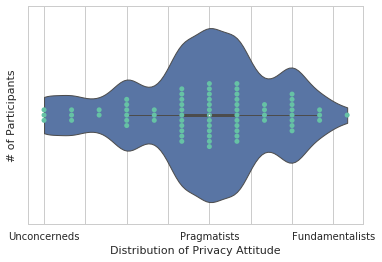
\includegraphics[width=1.0\columnwidth]{fig/privacy-attitude-distribution.png}
    
%     \begin{tikzpicture}

% \begin{axis}[
%     ybar,
%     % bar width=0.5,
%     % ymin=0,
%     xmin=1, xmax=5,
%     height=3cm, width=6cm,
%     xlabel={Privacy Attitude},
%     % ylabel={Society},
%     xtick = {1,2,3,4,5},
%     xticklabels={Unconcerned,,,, Concerned},
%     % yticklabel style={rotate=45},
%     ytick={1},
%     yticklabels={Participants},
%     enlarge x limits=0.03, % adjust space between axis edge and plot edge
%     ]
%     \addplot+[boxplot]
%  	table[y index=0]
%  	{./Chapter-5/data/privacy_profiles.csv};
 	
% \end{axis}
% \end{tikzpicture}
    
%      \caption{Distribution of privacy attitudes of the human-subject study participants.}
%      \label{fig:participants-privacy-distribution}
%  \end{figure}

Next, the participants completed two context-sharing surveys. 
In the first survey, they were given a list of contexts, as listed in Table~\ref{tab:places}, and their companions (alone, co-worker, family, friend, or crowd) in the given context, and were asked to select a sharing policy (share with all, share only with common friends, or share only with companions). In the second survey, participants were additionally informed of the values that are promoted or demoted on sharing and on not sharing the context, and were asked to select a context sharing policy accordingly. We use the first survey to engage and immerse the participants in various contextual scenarios, and the second to help them make informed decisions according to the values promoted or demoted in each context.

We use the privacy attitudes of the participants and the context sharing policies selected by the participants to create multiple artificial societies of stakeholders and to seed the simulation experiments described in Chapter~\ref{sec:results}. 

\section{Experiments and Results}
\label{sec:results}

We evaluate our research question via two experiments in which we simulate societies of \locationapp SIPAs who visit different places and may share their context. First, we experiment with a society of stakeholders with mixed privacy attitudes representing the attitudes of participants collected in the study described in Chapter~\ref{sec:survey}. Second, we experiment with three societies with a majority of privacy casual, conscientious, or cautious stakeholders, respectively.

Our results are stable with changes in the network size and the connectedness of a SIPA society. 

\subsection{Decision-Making Strategies}
\label{sec:decision-making-strategies}

As \locationapp SIPAs move between places and interact with each other, they make policy decisions that affect their stakeholders. To evaluate SIPAs designed via \frameworkAinur, we define four (\frameworkAinur and three baseline) policy decision-making strategies. 

\begin{description}
\item[S\fsub{\frameworkAinur}: \frameworkAinur.] The SIPA produces a context sharing policy using the VIKOR method rankings computed based on value preferences of its stakeholders.
\item[S\fsub{primary}: Primary user's preference.] The SIPA produces a context sharing policy based only on its primary stakeholder's value preferences. This is representative of how location sharing works today in social networking websites such as Facebook. 
\item[S\fsub{conservative}: Most privacy conservative policy.] The SIPA produces the least privacy violating, i.e., the most restrictive context sharing policy among the available alternatives based on its stakeholders' value preferences. It represents policy selection based on the least negative consequence. 
\item[S\fsub{majority}: Majority policy.] The SIPA produces the most common context sharing policy based on its stakeholders' value preferences. It represents policy selection based on majority voting. 
\end{description}

\subsection{Metrics}

For each SIPA interaction, we compute these measures:

\begin{description}
\item[Mean social experience,] the mean utility obtained by the society as a whole based on context sharing policy decisions. Higher is better.
\item[Best individual experience,] the maximum utility obtained by any of the SIPA's stakeholders during a single interaction. Higher is better.
\item[Worst individual experience,] the minimum utility obtained by any of the SIPA's stakeholders during a single interaction. The intuition behind choosing this measure to verify if a society supports Maximin \citep{Leben2017Rawls}. Higher is better. 
\item[Fairness,] the reciprocal of the difference between the best and the worst individual experience obtained by the SIPA's stakeholders during a single interaction. It is based on the dispersion of the experience yielded by SIPAs \citep{rawls1985justice}. Higher is better. 
% \item[Privacy violation] measures the extent to which a SIPA's policy violates its stakeholders' privacy. Lower is better.
% \hg{maybe change to the value gain of privacy? it's easier}
% \item[Social conflicts] measures the percentage of agents that find actions as compliant to their value preferences. 
\end{description}

\paragraph*{Computing Utility.} The utility that a SIPA obtains from a sharing policy in a certain context, whether to a primary or a secondary stakeholder, 
is a weighted sum of four numeric utility payoffs that the stakeholder perceive with respect to the four types of values considered in our example. We preset these numbers in a utility matrix such that they reflect a human-subject's preferences over these values. We assume that a stakeholder receives the maximum utility when the chosen sharing policy is the preferred one, and the utility decreases linearly when the policy chosen by a SIPA deviates from it. Table~\ref{tab:utlitymatrix} lists the preferred policies and utility numbers for each value of one human-subject in different contexts. 

\begin{table}[!htb]
\centering
\caption{Example numeric utility matrix for a stakeholder. }
\label{tab:utlitymatrix}
\begin{tabular}{lllcccc}
\toprule
\multirow{2}{*}{Place} & \multirow{2}{*}{Companion} & \multirow{2}{*}{Policy} & \multicolumn{4}{c}{Value}\\
\cmidrule{4-7}
& & & Pl & Pr & R & S\\
\midrule
\rowcolor{lightgray!50!}
Graduation & Family & All &1&0&1&0 \\ 
Conference & Co-workers & None &0&1&0&0 \\
\rowcolor{lightgray!50!}
Library & Friends & All &1&0&0&0 \\
Airport & Friends & Common &0&1&0&0 \\
\rowcolor{lightgray!50!}
Hiking & Alone & All &1&0&0&1 \\
Hurricane & Family & All &1&0&0&1 \\
\rowcolor{lightgray!50!}
Bar & Alone & None &0&2&0&0 \\
Rehab & Friends & None &0&2&0&0\\
\bottomrule
\multicolumn{7}{p{8cm}}{Pl, Pr, R, and S are pleasure, privacy, recognition, and security, respectively.}
\end{tabular}
\end{table}

\subsection{Hypotheses}

We propose the following hypotheses to evaluate our research question. We omit the corresponding null hypotheses for brevity. 

\begin{description}
\item[H\fsub{social}.] \frameworkAinur yields better mean social experience than baseline strategies. 
\item[H\fsub{best}.] \frameworkAinur yields higher best individual experience than baseline strategies. 
\item[H\fsub{worst}.] \frameworkAinur yields higher worst individual experience than baseline strategies. 
\item[H\fsub{fairness}.] \frameworkAinur yields higher fairness than baseline strategies. 
% \item[H\fsub{privacy}.] Policy decisions made by \frameworkAinur are less privacy violating than baseline strategies. 
% \item[H\fsub{conflict}.] Policy decisions made by \frameworkAinur are more compliant to value preferences of SIPA stakeholders compared to baseline strategies
\end{description}


\subsection{Experimental Setup}

% \nsa{Include how social experience is computed. Include utility matrix.}

We run simulations on a society of \locationapp SIPAs. All parameters described below are set empirically based on the human-subject study we conducted.

Specifically, we experiment on a society of 580 SIPAs, ten per study participant, each of which assumes the properties, including preferred choices and privacy attitude, of an actual study participant. In the default setting, which we use in the experiment with a mixed agent society, the SIPAs are mapped evenly to the participants. For each pair of SIPAs, their relationship is co-worker, friend, family (with equal probability), or strangers.
% with the probabilities of 10\%, 10\%, 10\%, and 70\%, respectively. 
Relationships are assigned at the beginning of the simulations such that they exhibit small world properties (degree: 10, rewiring prob: 0.05, edges: 3,445, clustering coefficient: 0.56, density: 0.014, average distance: 4.71) \citep{Watts+Strogatz-98}. 
% Figure~\ref{fig:smallworld-69d10p50} shows our experimental social network.

% \begin{figure}[!htb]
%     \centering
%     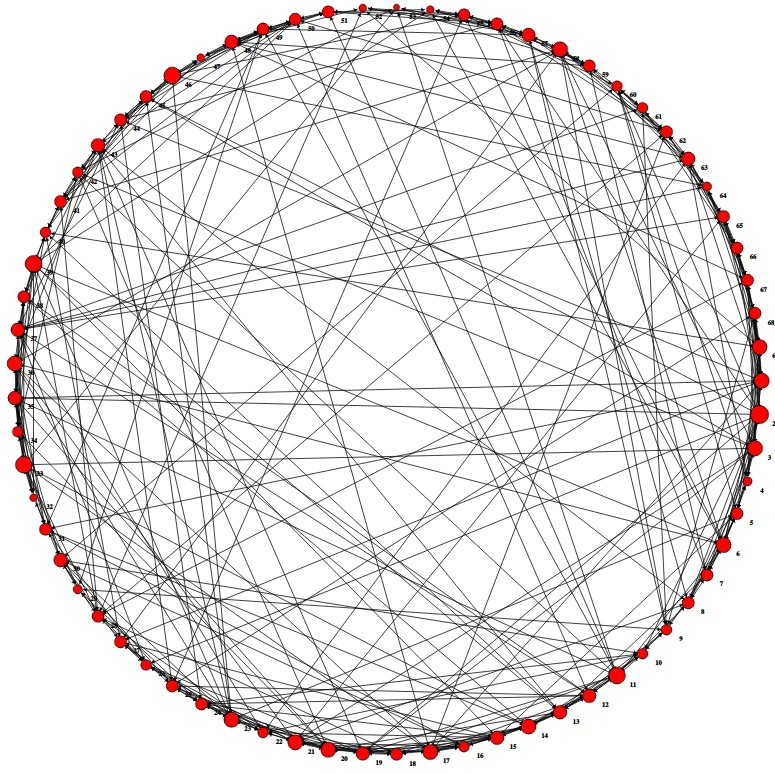
\includegraphics[width=0.7\columnwidth]{fig/smallworld-69d10p50.jpg}
%     \caption{The \emph{small-world} network of SIPAs.}
%     \label{fig:smallworld-69d10p50}
% \end{figure}

At each step in the simulation, each SIPA is at one of the eight places listed in Table~\ref{tab:places}. The SIPA moves after one step to another place with equal probability. A SIPA decides a context sharing policy based on the current place and the SIPA's stakeholders' privacy attitudes, value preferences, and decision-making strategy in Chapter~\ref{sec:decision-making-strategies}.  

% In each step, each agent has the probability of 2\% to be a primary stakeholder and check-in at a random context (from eight contexts listed in Table~\ref{tab:places}). If an agent decides to share context, it either tags no one, only family, only friends, only co-workers, or acquaintances with equal probabilities. Each acquaintance has the probability of 3\% of being tagged. If only tagging colleagues, friends or family, each acquaintance has the probability of 9\% of being tagged. A check-in policy is based on an agent's personality type and its policy decision-making strategy. 
% \nsa{Rewrite. From the above text it seems check-in and tagging actions are probabilistic and not deterministic based on VIKOR.}

% The primary stakeholder chooses a context sharing policy based on one of the decision-making strategies in Chapter~\ref{sec:decision-making-strategies}, and the average utility of each involved agent is calculated based on this policy. The utility that an agent receives is the weighted value gain of the four value types. We choose the weights based on the users' privacy attitudes. 

For each setting, we run the simulation 2,000 steps three times and report the mean social experience, the best individual experience, the worst individual experience, and fairness. We plot the mean social experience after every 100 steps in one run. 

\subsection{Experiment with Mixed Agent Society}

First, we experiment using the default settings as described above. The privacy attitude distribution of the mixed agent society mimics the privacy attitude distribution of our study participants  shown in Figure~\ref{fig:participants-privacy-distribution}.

To evaluate hypothesis H\fsub{social}, we compare the \fsl{mean social experience} obtained by SIPAs built according to the four decision-making strategies---S\fsub{\frameworkAinur}, S\fsub{primary}, S\fsub{conservative}, and S\fsub{majority}. Similarly, for H\fsub{best}, H\fsub{worst}, and H\fsub{fairness}, we compare the \fsl{best individual experience}, \fsl{worst individual experience}, and \fsl{fairness}, respectively, as yielded by these decision-making strategies. 

Table~\ref{tab:result-mixed} summarizes the results for the experiments with a mixed agent society.  It shows values for mean, best, and worst social experience, fairness, and p-values from the two-tailed paired t-tests comparing the mean social experience yielded by \frameworkAinur and by other strategies. Figure~\ref{fig:weighted-experience-plot} shows the mean social experience plots. 


\begin{table}[!htb]
\centering
\caption{Comparing social experience, best and worst individual experience, and fairness yielded by \frameworkAinur SIPAs using VIKOR vs other decision-making strategies in a society with mixed privacy attitudes.}
\label{tab:result-mixed}
\begin{tabular}{lrrrrr}
\toprule
Strategy & Mean & Best & Worst & Fairness & \fsl{p}\\%&Privacy\\
\midrule
\rowcolor{lightgray!50!}
S\fsub{\frameworkAinur} & \fbf{1.361} & 1.715& \fbf{0.767} & \fbf{1.05} & --\\%& 0.581\\
S\fsub{primary} & 1.286&1.789&0.579 & 0.83 & \textless0.01 \\%& 0.588\\
\rowcolor{lightgray!50!}
S\fsub{conservative} & 1.106&1.721&0.472 & 0.80 & \textless0.01 \\%& 0.682\\
S\fsub{majority} & 1.339 &\fbf{1.836}&0.570 & 0.78 & \textless0.01 \\%& 0.621\\
\bottomrule
\end{tabular}
\end{table}



% \begin{figure}[!tb]
%     \centering
%     \begin{tikzpicture}
%     \begin{axis}[
%     title={},
%     height=4cm,
%     width=5cm,
%     xlabel={Time in 100 steps},
%     ylabel={Experience},
%     xtick={500,1000,1500,2000},
%     xticklabels={5,10,15,20},
%     xmin=0,xmax=2100,
%     ymin=0.3,ymax=1.7,
% %     legend pos=south east,
%     legend style={at={(1.7,0.3)}, anchor=east, font=\tiny},    
%     ]
%     \addplot +[mark=none] table [x=tick, y=ainur, col sep=comma]
%     {./Chapter-5/data/basicresults.csv};
%     \addplot +[mark=none] table [x=tick, y=primary, col sep=comma]
%     {./Chapter-5/data/basicresults.csv};
%     \addplot +[mark=none] table [x=tick, y=conservative, col sep=comma]
%     {./Chapter-5/data/basicresults.csv};
%     \addplot +[mark=none] table [x=tick, y=majority, col sep=comma]
%     {./Chapter-5/data/basicresults.csv};
%     \legend{S\fsub{\frameworkAinur},S\fsub{primary},S\fsub{conservative},S\fsub{majority}}
%     \end{axis}
%     \end{tikzpicture}
%     \caption{\frameworkAinur vs other strategies' social experience}
%     \label{fig:experience-plot}
% \end{figure}

\begin{figure}[!tb]
    \centering
    \begin{tikzpicture}
    \begin{axis}[
    title={},
    height=7cm,
    width=7cm,
    xlabel={Time in 100 steps},
    ylabel={Social Experience},
    xtick={500,1000,1500,2000},
    xticklabels={5,10,15,20},
    xmin=0,xmax=2100,
    ymin=0.7,ymax=1.7,
%     legend pos=south east,
    % legend style={at={(1.8,0.3)}, anchor=east},
    legend style={at={(0.5,-0.3)},anchor=north,},
    legend columns=4, 
    ]
    \addplot +[mark size=1,] table [x=tick, y=ainur, col sep=comma]
    {./Chapter-5/data/weightedresults.csv};
    \addplot +[mark size=1, densely dashed] table [x=tick, y=primary, col sep=comma]
    {./Chapter-5/data/weightedresults.csv};
    \addplot +[mark size=1.5, green!30!black, dashed, mark=diamond*] table [x=tick, y=conservative, col sep=comma]
    {./Chapter-5/data/weightedresults.csv};
    \addplot +[mark size=1.5, densely dashdotted] table [x=tick, y=majority, col sep=comma]
    {./Chapter-5/data/weightedresults.csv};
    \legend{S\fsub{\frameworkAinur},S\fsub{primary},S\fsub{conservative},S\fsub{majority}}
    \end{axis}
    \end{tikzpicture}
    \caption{\frameworkAinur vs other strategies' social experience.}
    \label{fig:weighted-experience-plot}
\end{figure}


We observe that \frameworkAinur yields better mean social experience than  other decision-making strategies. Although the mean best individual experience obtained by \frameworkAinur SIPA stakeholders is not the largest, they yield the highest mean worst individual experience and fairness. 
These results indicate that \frameworkAinur yields solutions such that each companion is treated fairly, and thus \frameworkAinur SIPAs act ethically. Thus, the null hypotheses corresponding to H\fsub{social}, H\fsub{best}, H\fsub{fairness} are rejected.


\subsection{Experiments with Majority Privacy Attitudes}
Next, since our study sample may not be representative of privacy attitudes of the general population, we create three artificial societies with stakeholders having different distributions of privacy attitudes from the study data. 
We experiment with societies that are dominated by privacy casual, conscientious, and  cautious stakeholders. Boxplots in Figure~\ref{fig:privacy-distribution-experiment} show the distributions of privacy attitudes of the stakeholders in these artificial societies. 

\begin{figure}[!htb]
\centering
\begin{tikzpicture}
\begin{axis}[
    % title={Privacy attitude distribution of three societies},
    % ybar,
    % bar width=0.5,
    % ymin=0,
    xmin=1, xmax=5,
    height=7cm, width=7cm,
    xlabel={Privacy Attitude},
    % ylabel={Society},
    xtick = {1,5},
    xticklabels={Unconcerned, Concerned},
    % yticklabel style={rotate=45},
    ytick={1,2,3},
    yticklabels={Cautious, Conscientious, Casual},
    enlarge x limits=0.03, % adjust space between axis edge and plot edge
    ]
    \addplot+[boxplot]
 	table[y index=0]
 	{./Chapter-5/privacy_attitude/fundamentalist_privacy_attitude.csv};
 	\addplot+[boxplot]
 	table[y index=0]
 	{./Chapter-5/privacy_attitude/pragmatic_privacy_attitude.csv};
 	\addplot+[boxplot]
 	table[y index=0]
 	{./Chapter-5/privacy_attitude/unconcerned_privacy_attitude.csv};
%  	\addplot+[green!50!black,boxplot,mark options={fill=green!50!black}]
%  	table[x expr=\coordindex, y index=0]
%  	{./Chapter-5/data/privacy_profiles.csv};
\end{axis}
\end{tikzpicture}
\caption{Privacy attitude distributions for artificial societies of cautious, conscientious, and casual stakeholders.}
\label{fig:privacy-distribution-experiment}
\end{figure}

Table~\ref{tab:result-privacy} summarizes the results for the experiments with privacy cautious, conscientious, and casual societies. Figure~\ref{fig:experience-plot+privacy} shows the social experience plots for these experiments.

\begin{figure}[!htb]
    \centering
    \begin{tikzpicture}
    \begin{axis}[
    legend columns=-1,
    legend entries={S\fsub{\frameworkAinur},S\fsub{primary},S\fsub{conservative},S\fsub{majority}},
    legend to name=named,
    title={Privacy Cautious Society},
    height=6cm,
    width=7cm,
    % xlabel={Time in 100 steps},
    ylabel={Social Experience},
    xtick={500,1000,1500,2000},
    xticklabels={5,10,15,20},
    xmin=0,xmax=2100,
    ymin=0.7,ymax=1.7,
    ]
    \addplot +[mark size=1] table [x=tick, y=ainur, col sep=comma]
    {./Chapter-5/data/funresults.csv};
    \addplot +[mark size=1, densely dashed] table [x=tick, y=primary, col sep=comma]
    {./Chapter-5/data/funresults.csv};
    \addplot +[mark size=1.5, green!30!black, dashed, mark=diamond*] table [x=tick, y=conservative, col sep=comma]
    {./Chapter-5/data/funresults.csv};
    \addplot +[mark size=1.5, densely dashdotted] table [x=tick, y=majority, col sep=comma]
    {./Chapter-5/data/funresults.csv};
    \end{axis}
    \end{tikzpicture}
%

%     
    \begin{tikzpicture}
    \begin{axis}[
    title={Privacy Conscientious Society},
    height=6cm,
    width=7cm,
    % xlabel={Time in 100 steps},
%     ytick={},
    ylabel={Social Experience},
    xtick={500,1000,1500,2000},
    xticklabels={5,10,15,20},
    xmin=0,xmax=2100,    ymin=0.7,ymax=1.7,
%     legend pos=south east,
%     legend style={at={(0.5,-0.1)}, anchor=north, font=\tiny},
    legend style={at={(0.5,-0.2)},anchor=north,},
    legend columns=2 
    ]
    \addplot +[mark size=1] table [x=tick, y=ainur, col sep=comma]
    {./Chapter-5/data/pragresults.csv};
    \addplot +[mark size=1, densely dashed] table [x=tick, y=primary, col sep=comma]
    {./Chapter-5/data/pragresults.csv};
    \addplot +[mark size=1.5, green!30!black, dashed, mark=diamond*] table [x=tick, y=conservative, col sep=comma]
    {./Chapter-5/data/pragresults.csv};
    \addplot +[mark size=1.5, densely dashdotted] table [x=tick, y=majority, col sep=comma]
    {./Chapter-5/data/pragresults.csv};
    % \legend{S\fsub{\frameworkAinur},S\fsub{primary},S\fsub{conservative},S\fsub{majority}}
    \end{axis}
    \end{tikzpicture}
%

%
    \begin{tikzpicture}
    \begin{axis}[
    title={Privacy Casual Society},
    height=6cm,
    width=7cm,
    xlabel={Time in 100 steps},
%     ytick={},
    ylabel={Social Experience},
    xtick={500,1000,1500,2000},
    xticklabels={5,10,15,20},
    xmin=0,xmax=2100,
    ymin=0.7,ymax=1.7,
%     legend pos=south east,
    % legend style={at={(1.8,0.3)}, anchor=east},  
    legend style={at={(0.5,-0.2)},anchor=north,},
    legend columns=4 
    ]
    \addplot +[mark size=1] table [x=tick, y=ainur, col sep=comma]
    {./Chapter-5/data/unconcernedresults.csv};
    \addplot +[mark size=1, densely dashed] table [x=tick, y=primary, col sep=comma]
    {./Chapter-5/data/unconcernedresults.csv};
    \addplot +[mark size=1.5, green!30!black, dashed, mark=diamond*] table [x=tick, y=conservative, col sep=comma]
    {./Chapter-5/data/unconcernedresults.csv};
    \addplot +[mark size=1.5, densely dashdotted] table [x=tick, y=majority, col sep=comma]
    {./Chapter-5/data/unconcernedresults.csv};
    % \legend{S\fsub{\frameworkAinur},S\fsub{primary},S\fsub{conservative},S\fsub{majority}}
    \end{axis}
    \end{tikzpicture}
    \\
    \ref{named}
    \caption[\frameworkAinur vs other strategies: Social experience in different societies]{Comparing \frameworkAinur with other strategies with respect to social experience in societies based on privacy attitudes.}
    \label{fig:experience-plot+privacy}

\end{figure}


\clearpage
\newpage
\KOMAoptions{paper=landscape,pagesize}
\recalctypearea

% \begin{sidewaystable*}[ph!]
\begin{table}[ht!]
%\centering
\caption[\frameworkAinur vs other strategies: Social experience and fairness in different societies]{Comparing social experience, best and worst individual experience, and fairness yielded by \frameworkAinur SIPAs using VIKOR with other decision-making strategies in societies based on majority privacy attitudes.}
\label{tab:result-privacy}
%% \begin{tabular}{lr@{~~}r@{~~}r@{~~}r@{~~}r@{~~}r@{~~}r@{~~}r@{~~}r@{~~}r@{~~}r@{~~}r@{~~}}
\begin{tabular}{l r r r r r r r r r r r r}
\toprule
\multirow{2}{*}{Strategy}& \multicolumn{4}{c}{Cautious} & \multicolumn{4}{c}{Conscientious} &\multicolumn{4}{c}{Casual}\\
\cmidrule(lr){2-5} \cmidrule(lr){6-9} \cmidrule(lr){10-13}
& Mean & Best & Worst & Fairness & Mean & Best & Worst & Fairness & Mean & Best & Worst & Fairness\\
\midrule
\rowcolor{lightgray!50!}
S\fsub{\frameworkAinur} & 1.535 & 1.664 & \fbf{1.233} & \fbf{2.27} & \fbf{1.329} & 1.531 & \fbf{0.867} & \fbf{1.51} & \textbf{1.242} & 1.457 & \fbf{0.768} & \fbf{1.45}\\
S\fsub{primary} & 1.506 & 1.766  & 1.082 & 1.46 & 1.253 & 1.592 & 0.679 & 1.10 & 1.129 & 1.466 & 0.584 & 1.13\\
\rowcolor{lightgray!50!}
S\fsub{conservative} & 1.366 & 1.745 & 1.059 & 1.46 & 1.093 & 1.519 & 0.608 & 1.10 & 0.870 & 1.338 & 0.454 & 1.34\\
S\fsub{majority} & \fbf{1.551} & \fbf{1.858} & 1.007 & 1.18 & 1.318 & \fbf{1.699} & 0.575 & 0.89 & 1.176 & \fbf{1.534} & 0.518 & 0.98\\
\bottomrule
\end{tabular}
% \end{sidewaystable*}
\end{table}

\clearpage
\newpage
\KOMAoptions{paper=portrait,pagesize}
\recalctypearea

\subsubsection{Privacy Cautious Society}

We find that, although \frameworkAinur yields the second best mean social experience next to the majority strategy, the worst individual experience yielded by \frameworkAinur is the maximum. For fairness, \frameworkAinur has the highest outcome. Thus, the null hypotheses related to H\fsub{worst} and H\fsub{fairness} are rejected. 

\subsubsection{Privacy Conscientious Society}

Here, \frameworkAinur yields the best mean social experience and maximizes the worst individual experience while giving the fairest solutions. Hence, the null hypotheses related to H\fsub{worst} and H\fsub{fairness} are rejected.

\subsubsection{Privacy Casual Society}

Again, \frameworkAinur yields the best mean social experience while giving the fairest solutions with the highest worst individual experience; thus, the null hypotheses related to H\fsub{worst} and H\fsub{fairness} are rejected. 

\subsection{Threats to Validity and Mitigation}

We identify and mitigate three threats. 
%
The first threat concerns simulation as an evaluation methodology. Obtaining data with actual human users' preferences and attitudes is challenging. And more so, testing a SIPA's adaptation
in all possible social contexts would be infeasible. Simulation provides an excellent avenue to overcome that challenge. Our simulation results are grounded in data obtained from users. 

Second, in reality users may perceive social experience differently than when completing a survey. Self-reported attitudes are unreliable and indirect methods may yield better quality data. To mitigate the threat associated with self-reported attitudes, we employ context check-in scenarios in which participants immerse themselves and accordingly provide check-in policies.

Third, the privacy attitudes in our survey sample may not be representative actual population. Even with a survey on a larger scale, imagining all possible contexts is challenging. To mitigate this threat, we conduct multiple experiments with societies having different privacy attitudes. 

\section{Discussion}
\label{sec:discussion}
We advance the science of privacy by tackling a nuanced notion of privacy---understood as an ethical human value. We envision a society of socially intelligent agents participating in creative processes while they serve as technical components of a social machine. We borrow principles from operational research to guide these agents in ethical decision-making.

Specifically, we address the problem of designing an ethical personal agent that understands the value (including privacy and security) preferences of all its stakeholders (and not just its primary human user), and reasons about those preferences when acting on behalf of or suggesting actions to its user. 

% We develop \frameworkAinur, a framework to design such ethical personal agents. \frameworkAinur incorporates the VIKOR method to produce ethically fair actions in scenarios where norms or value preferences of multiple stakeholders conflict. We evaluate \frameworkAinur via simulation experiments seeded using crowdsourced data and find that \frameworkAinur yields a fair  social experience to all its stakeholders.

\subsection{Other Related Works}

We now discuss some other relevant related works. 

\subsubsection{Norms, Values, and Privacy in Multiagent Systems}
The contributions of this paper relate to the extensive work on norms and values, as well as privacy in the multiagent systems community.

\citet{Cranefield+16:norm-identification} provide a machine learning approach through which agents can identify its societal norms based on their observations of behavior and sanction in a society. 
\citet{IJCAI-18:Poros} develop socially intelligent agents who apply norms to provide privacy assistance to their users. Their notion of privacy implicitly incorporates values by considering not only confidentiality but higher-level concerns such as disapprobation and avoiding infringing into others' space. 
However, \citet{IJCAI-18:Poros}'s agents seek to maximize the social experience of their respective users. Maximizing social experience may not translate to fairness as we observed in experiments with privacy cautious society where S\fsub{majority} yields maximum social experience but least fairness. 
\frameworkAinur's focus is to balance the needs of primary and secondary users. 

\citet{Ajmeri-AAMAS17-Arnor} provide an approach for engineering agents who promote privacy. Their approach lacks constructs to model stakeholders' values. Our framework, \frameworkAinur, including understanding of value preferences to aid group decision-making, and its evaluation are novel.
% 
Additionally, in contrast to all these works, the present work is focused on values. It is empirically grounded in data from users, and it takes into account group decision-making.

\citet{Borning-CHI2012-VSD} address Value Sensitive Design and suggest that researchers respect differences in user's views on human values widely across cultures and contexts. 

\citet{anderson-2015-ethical}, however, assert that autonomous systems should be guided by ethical consensus determined by ethicists in different areas. They propose a case-supported paradigm to help ensure autonomous systems that make decisions only when there is a consensus on what is ethically correct. \frameworkAinur SIPAs select ethically appropriate actions by aggregating value preferences of all its users.

% may need rephrasing
\citet{Bench-Capon-ail2017} argue for the need of value-based reasoning in agents, especially when norms should be violated. They propose that agents keep track of the preference ordering of values. However, they posit that rules are made to be broken, and consider only the circumstances where norms should be violated. We argue that agents should model and resolve conflicts among norms based on stakeholders' views on values as well as social contexts. Under different social contexts, stakeholders' preferences of values may also vary. 

\citet{Cranefield-ijcai17-value+bdi} describe a mechanism of value-based reasoning for BDI (Belief-Desire-Intention) agents. They argue that decision-making by agents in normative systems, such as the selection of norms, is indirectly influenced by the value system, and therefore do not model norms in their approach. 
%\hg{we argue that norms should be kept} 
However, without norms, agents would need a complete understanding of human values to make morally correct decisions, which is difficult to realize. 

\citet{dignum-ijcai17-responsible} argues for the need for AI reasoning to take into account societal values because autonomous AI systems increasingly affect our lives. Dignum proposes several approaches to responsibility in AI design considering human values. 
% \hg{no experiments or evaluations. This paper is more like an argument than research. Maybe move to introduction}

\citet{Kayal-TOIT18} propose an automatic value-based model for resolving conflicts between norms, especially social commitments, in multiagent systems. Their results from a user study provide evidence that values can influence, and therefore could be used to predict, users' preferences when resolving conflicts. \frameworkAinur supplements Kayal {\etal}'s model by providing constructs and mechanisms to develop value-driven ethical SIPAs and thus, goes beyond conflict resolution. 
\citet{Serramia+18:values} show how to incorporate values along with norms in a heuristic decision-making framework.

\subsubsection{Value Alignment in Artificial Intelligence}

Some recent works focus on value alignment of artificial intelligence systems and how agents can learn human values correctly. 
\citet{RiedlHarrison2016Stories} argue that it is not easy for developers to exhaustively enumerate human values, and propose that agents use sociocultural knowledge embedded in stories, such as crowdsourced narratives, to learn human values. 
\citet{arnold-2017-value} address how inverse reinforcement learning (IRL) can be used in value alignment, and propose a hybrid approach for reasoning about moral norms combining IRL and logical representations of norms. \frameworkAinur SIPAs can adopt such approaches to learn value preferences of their users. 

% \hg{They do not explicitly talk about values. more in the ``thou shalt be good'' sense}
% Soares \citep{Soares2016ValueLearning} argues for the difficulty of the value learning problem, and that agents should model and act according to the preferences of their stakeholders. 

\subsubsection{Understanding Privacy Preservation}

Many researchers focus on understanding the growing aspects of privacy, especially with new information technologies being constantly developed. 
% 
\citet{smith2007privacy} survey privacy in e-commerce both from a consumer's point of view and a business' point of view. 
Consumers either view privacy as a human value or relate it to economics of information. 
In either case, they prefer control of their personal information (or economic property). 
Businesses have lost market share or income because of privacy concerns, 
and thus are leaning toward giving consumers control over their personal information to alleviate privacy concerns and gain trust.  
Smith and Shao also survey privacy enhancing technologies and suggest anonymising technologies, while effective in several cases, may not be always viable or desirable. 
\citet{Acquisti-2017-Nudges+Privacy+Security} review research on assisting individuals' online privacy and security choices. 
They discuss the merits and limits of interventions that nudge users toward making the ``right'' choices, balancing revelation and protection of data. 

\subsubsection{Privacy-Preserving Applications}

Other recent studies focus on the designing privacy-preserving applications. 
% 
\citet{Campagna-WWW2017-Almond} present an architecture of a privacy-preserving virtual assistant for online services and the Internet of Things (IoT) that follows natural language commands for trigger-action tasks. They state that virtual assistants need to handle all of the users' personal information in order to comprehensively serve them. To preserve privacy, they propose a system that can run locally to store the information. 
Whereas \citet{Campagna-WWW2017-Almond}'s treatment of privacy is limited to information disclosure, we tackle nuanced notions of privacy understood as an ethical value.

\citet{Barry-CHI2017-EthicalDesign} propose a framework that adopts an Aristotelian virtue ethics concept, phronesis, for developing ethical mobile health apps. Phronesis describes the practical wisdom of gathering experience in a specific context. \citet{Barry-CHI2017-EthicalDesign} claim that applications with phronesis learn contextual client knowledge, and therefore make right choices that inherently involve ethical reflection. However, their design does not address conflicts of different choices and priorities, which are common in social settings. 

%\subsection{Future Directions}
%A first significant direction is to empirically evaluate the effectiveness of
%\frameworkAinur via a developer study. 
%A second direction is to develop a SIPA similar to the \locationapp SIPA using \frameworkAinur 
%as a privacy enhancing technology that learns value preferences of its stakeholders, 
%and selects ethically appropriate policies.
%A third direction is to incorporate argumentation and value-based 
%reasoning to model and reason about value preferences. 


% \mps{George Vouros,
%   Julian Padget,
% %  Marco Montali,
%   Michael Rovatsos,
% %  Stefania Costantini,
% %  Marco Alberti,
% }

% \mps{
%   Birna, 
%   Brian Logan,
%   Natasha Alechina,
%   Juan Antonio Rodriguez Aguilar,
% %  Gita Sukthankar,
% %  Marina de Vos,
%   Leon van der Torre,
%   Stephen Cranefield,
%   Virginia Dignum,
%   Eva Onaindia,
% %  Simon Parsons,
% %  Hasan Davulcu,
% %  Thomas  Agotnes,
%   Kiran  Lakkaraju,
% %  Kobi  Gal,
% %  Wlodek  Zadrozny,
% %  Yves  Lesperance,
%   Franziska Klugl,
% %  Federico Cerutti, 
% %  Francois Schwarzentruber,
% %  Frans Oliehoek,
% %    Renata  Wasserman,
% }

%\mps{Has Pasotti appeared (2016)?} \nsa{Can't find a formal proceedings of NorMAS where this appeared.}
%\mps{The proc is here \url{https://link.springer.com/book/10.1007\%2F978-3-319-66595-5} (remove backslash) but no Pasotti}\mps{remove the "to appear" and remove mention of Springer; you can ask Birna too but time is tight now and this is a low priority action} \nsa{Updated}